\begin{figure}[h]
     \centering
     \begin{subfigure}[h]{0.5\textwidth}
         \centering
         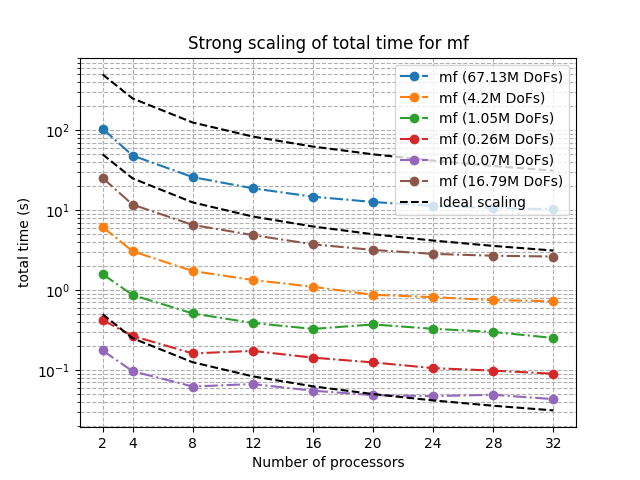
\includegraphics[width=\textwidth]{figure/strong_mf_total.png}
         \caption{Matrixfree}
     \end{subfigure}
     \hspace*{-0.4cm}
     \begin{subfigure}[h]{0.5\textwidth}
         \centering
         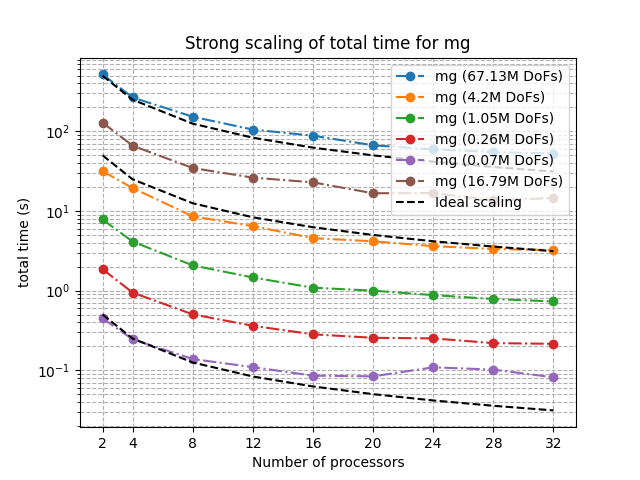
\includegraphics[width=\textwidth]{figure/strong_mg_total.png}
         \caption{Matrixbased}
     \end{subfigure}
     \caption{Total time scaling for both matrixfree and matrixbased multigrid solvers. Strong scaling can be compared with the reference lines, weak scaling can be assessed knowing that each plot differs quadruplicates the problem size.}
     \label{fig:strong_mg_mf}
\end{figure}
